\documentclass[a4paper,12pt]{scrartcl}
 
\usepackage[utf8]{inputenc} 
\usepackage[ngerman]{babel}
\usepackage[T1]{fontenc}
\usepackage{amsmath}
\usepackage{hyperref}
\usepackage{tikz}
\usepackage{svg}
\usetikzlibrary{automata,positioning}
\usepackage{pdfpages}
\usepackage{listings}

\bibliographystyle{unsrt}

\hypersetup{
    colorlinks,
    citecolor=black,
    filecolor=black,
    linkcolor=blue,
    urlcolor=black
}



\title{}


\author{Johannes Bohlig}

\date{\today}


\begin{document}

\tableofcontents

\pagebreak

\section{Einleitung}

Anbieter von Cloud-Services haben den Anspruch, möglichst geringe und kurze Ausfallzeiten mit ihren Services zu erreichen. Um eine maximal lange, störungsfreie Servicelaufzeit zu erreichen, ist es notwendig jederzeit den Servicestatus einsehen und mögliches Fehlverhalten frühzeitig erkennen zu können. 
Da für eine dauerhafte Kontrolle eines Services ein oder sogar mehrere Mitarbeiter benötigt würden, welche eine eintönige Kontrollaufgabe übernehmen müssten, ist es sinnvoll möglichst viele Teile der Kontrolle zu automatisieren. Diese Automatisierung bringt einerseits den Vorteil der Kosteneinsparung, da keine Mitarbeiter für diese Aufgabe benötigt werden und andererseits einen Geschwindigkeitsvorteil durch die wesentlich geringere Reaktionszeit, die durch die Geschwindigkeit von Computern gegenüber dem Menschen einhergeht.\\
Hierbei sollen vor allem Engpässe bei Ressourcen ausfindig gemacht werden, sowie Anomalien, also Fehlverhalten, in einzelnen Komponenten der Infrastruktur gefunden und behoben werden, bestenfalls noch bevor sich größere Auswirkungen auf die restlichen Komponenten ergeben.
Sofern Ressourcenengpässe, also hohe Last, auftritt und dies frühzeitig erkannt wird, können einzelne Services gezielt skaliert und so Beeinträchtigungen auf die Funktion verhindert werden. Da Engpässe oft temporär auftreten, werden Services sowohl hoch- als herunterskaliert um so immer die ideale Zahl an Ressourcen bereitgestellt.
Des Weiteren soll Fehlverhalten detektiert werden. Dies liegt dann vor, wenn hohe Ressourcenlast ohne erkennbaren Grund vorliegt. Das wäre beispielsweise dann der Fall, wenn die Prozessorlast oder Speicherlast eines Services auf einem sehr hohen Wert läuft, gleichzeitig aber keine hohe Netzwerklast durch Nutzer vorliegt, die dieses Verhalten begründet. In diesem Fall kann von einer anomalen Funktion ausgegangen und ein Service neu, im besten Fall unterbrechungsfrei, bereitgestellt werden. \\
Um eine automatisierte Erkennung zu ermöglichen, werden Daten sog. Metriken benötigt, die eine Entscheidung auf Basis des vorliegenden Verhaltens treffen lassen. Metriken müssen erhoben und ausgewertet werden, um eine Aktion aus ihnen schließen zu können, welche die vorliegende Anomalie oder den vorliegenden Engpass beheben kann.\\
Die erhobenen Metriken müssen einerseits für Menschen lesbar sein, um aktuelle Zustände widerspiegeln und entsprechend darauf reagieren zu können, andererseits ebenso für Computer auswertbar sein, um die Automatisierung durch diese zu ermöglichen.\\
Neben der Möglichkeit automatisierte Aktionen auszuführen, ist es auch sinnvoll entsprechende verantwortliche Administratoren über das Fehlverhalten in Kenntnis zu setzen und diese zu benachrichtigen, um ihnen die Möglichkeit zu geben dem Verhalten auf den Grund zu gehen.\\
Diese Arbeit setzt sich das Ziel die Durchführbarkeit der automatisierten Anomalie- und Engpasserkennung nachzuweisen und die erste Implementierung innerhalb eines schon bestehenden Kubernetes-Clusters. 
Im Rahmen dieser Arbeit werden die passenden Komponenten gewählt, die zur Umsetzung der Anforderungen benötigt werden, die Infrastruktur geplant, erstellt und die korrekte Funktion evaluiert.\\
Des Weiteren wird die Relevanz verschiedener erhobener Metriken in Bezug auf ihre Verwendbarkeit beim automatisierten Detektieren von Anomalien und Engpässen dargestellt und geklärt.\\
Es werden die weit verbreiteten Tools Prometheus und Grafana verwendet und durch Eigenentwicklungen ergänzt und so eine Infrastruktur geschaffen, welche die Anforderungen erfüllen kann.

\subsection{Struktur}

Diese Arbeit ist in neun Kapitel strukturiert. Im zweiten Kapitel werden die Grundlagen und für das Verständnis der weiteren Arbeit benötigtes Wissen vermittelt. Das Kapitel vermittelt grundlegendes Wissen zu den verwendeten Tools. Im dritten Kapitel wird der Status Quo der Technik ermittelt und somit die technische Ausgangslage der Arbeit geklärt. Mit dem vierten Kapitel beginnt der praktische Teil des Projekts. Am Anfang dessen steht die Vorgehensweise beim Aggregieren von Daten aus einem Kubernetes-Cluster. Nachdem Daten aggregiert wurden, müssen diese verarbeitet und ausgewertet werden. Das Vorgehen hierbei wird in Kapitel fünf erläutert. Die ausgewerteten Daten haben den Zweck automatisierte Aktionen auszulösen. Wie passende Aktionen gewählt und angewandt werden, damit befasst sich das sechste Kapitel.
Hier werden verwendete Komponenten, Architektur, Aktionen, Regeln sowie die passende Programmiersprache erläutert. Nachdem die geplanten Features implementiert sind, müssen diese auf ihre korrekte Funktion getestet werden. Im siebten Kapitel wird geklärt, wie die korrekte Funktion evaluiert wird, wie der Messaufbau gestaltet wurde und welche Komponenten auf welche Art und Weise getestet wurden.\\
Nach der Evaluation werden die Ergebnisse der Arbeit diskutiert. Hier werden Fragen geklärt  ob alle Ziele erreicht wurden oder aus welchem Grund Entscheidungen getroffen wurden. Diese und weitere Fragen werden in der Diskussion in Kapitel acht diskutiert.\\
Zum Schluss, in Kapitel neun, wird ein Fazit aus dem zurückliegenden Projekt gezogen und ein möglicher Ausblick in die Zukunft gestellt.

\pagebreak

\section{Grundlagen}
\subsection{Kubernetes}

Kubernetes, kurz "k8s", ist eine ursprünglich von Google entwickelte, mittlerweile aber quelloffene Software zur Orchestrierung und Deployment von containerisierten Anwendungen. Seit seiner Einführung 2014 hat Kubernetes ein starkes Wachstum erlebt und ist zum Quasistandard bei der Entwicklung von Cloud-Native Applikationen geworden.
Diese Übersicht der Grundlagen spricht die für dieses Projekt benötigten Komponenten an, für weitergehende Informationen gibt es die Dokumentation[Referenz auf Kube-Doku]\\

Die Relevanz von Kubernetes lässt sich an der halbjährlichen Befragung der Community der Cloud-Native Computing Foundation ablesen:
In der Umfrage stellte sich heraus, dass über 78 Prozent der 1337 Befragten Kubernetes verwendet.[Umfrage CNCF 2020 ergänzen]\\


Kubernetes ist eine mittlerweile bewährte Infrastruktur und bietet Software die nötig ist um zuverlässige und skalierbare verteile Systeme zu entwickeln. \cite{Burns.2019} \\
\subsubsection{Master Worker Prinzip}
Der Zweck eines Kubernetes-Clusters besteht darin viele, einzelne Computer als eine einzige Einheit zusammenarbeiten zu lassen.
Ein Cluster besteht aus zwei verschiedenen Arten von Komponenten, die zusammenarbeiten:
dem Node und dem Master.
Der Master stellt den Verwalter im Cluster dar. Er koordiniert alle Vorgänge, trifft also Entscheidungen die von globaler Bedeutung für das gesamte Cluster sind. Beispielsweise startet er Komponenten oder schaltet sie ab, ist aber auch für Tasks wie die Zeitplanung zuständig. Er wird über die Kubernetes-API angesprochen und steht in direkter Verbindung mit den Nodes.\cite{.20200530T15:19:3404:00} \cite{.20200316T05:14:35+01:00}
Nodes wiederum stellen die Arbeiter dar, weshalb sie auch "worker" genannt werden. Deren Aufgaben bestehen darin Pods[siehe Relevante Komponenten] aufrecht zu erhalten und die Laufzeitumgebung bereitzustellen. Nodes halten auch die Container-Runtime bereit, welche dafür zuständig ist Containerisierte Anwendungen auszuführen und so das verteilen einer Anwendung auf beliebige Hardware möglich macht.

<evtl. hier nochmal Grafik Master/Node>


\begin{figure}[htbp]
  \centering
  \input{KubernetesBasic.pdf_tex}
  \caption{einfache Darstellung eines Kubernetes-Cluster (eigene Zeichnung)}
\end{figure}

\pagebreak

\subsubsection{Relevante Komponenten}

Kubernetes bietet eine Vielzahl von Komponenten für unterschiedliche Aufgaben. Die für dieses Projekt Relevanten werden hier erklärt:

\begin{description}

\item [kubelet]: \\
Der kubelet ist der primäre 'node-agent'. Er ist dafür zuständig die Nodes beim Kubernetes API-Server zu registrieren. Des Weiteren verwaltet er Pods anhand einer Podspezifikation(PodSpec) und sorgt dafür, dass die Pods im Rahmen der Spezifikation "gesund" laufen.\\
Über den kubelet können diverse Metriken gesammelt werden, die über den Status des Nodes oder der darin laufenden Pods und Container Auskunft geben.\\

\end{description}

Kubernetes bietet verschiedene Organisiationskonzepte mit deren Hilfe sich die Kubernetes-Struktur umsetzen lässt, die für dieses Projekt wichtigsten werden im Folgenden erläutert:

\begin{description}

\item [Pod]:\\
Ein Pod ist eine 'execution unit' und repräsentiert einen Prozess, der in einem Cluster läuft. Ein Pod kapselt einen oder mehrere Anwendungs-Container, ein eigener Speicherbereich, eine eigene IP-Adresse sowie dessen Konfigurationsoptionen.
Die meistverwendete Container-Runtime ist,wie auch in diesem Projekt, Docker, es gibt aber auch Unterstützung für Weitere wie beispielsweise Rocket.\\
\item [Deployment]:\\
Das Deployment ist eine Beschreibung des Zustands, in dem Pods ausgeliefert werden sollen. Hier werden beispielsweise der Name, Namensraum, Ressourcenlimits oder auch die Größe der Skalierung definiert.
\item [Service]:\\
Nach der offiziellen Kubernetes-Dokumentation sind Services Eine "abstrakte Möglichkeit, eine Anwendung, die auf einer Reihe von Pods läuft, als Netzwerkdienst bereitzustellen".
Kubernetes Pods können dynamisch in ihrer Anzahl skalieren und so auch ihre IP-Adresse wechseln. Daher ist es sinnvoll die Pods über einen Service anzusprechen, der mit einem DNS ähnlichen System funktioniert und so ein Deployment über einen lesbaren Namen ansprechbar macht. 
\item [kubectl]:\\
kubectl ist eine Kontrollanwendung für Kubernetes. Es ist eine direkte Schnittstelle zwischen User und dem Kubernetes API-Server und kann mittels Konsolenbefehlen bedient werden. Das Tool stellt eine einfache Möglichkeit zur Bedienung des Kubernetes-Clusters dar. \\

\end{description}

Kubernetes bietet systemseitig Funktionen, die beim ermitteln von Cluster- und Systeminformationen helfen, eine davon ist der cAdvisor
 
\begin{description} 
\item [cAdvisor]:\\
Da Container von sich aus keine Informationen zu ihrem Ressourcenstatus nach außen preisgeben oder exportieren, bedarf es eines Hilfsmittels, das genau dies macht.
cAdvisor(Container Advisor) ist ein Daemon, der Ressourcen-Informationen aus Containern sammelt, verarbeitet und exportiert.\cite{.20200704T23:29:24.000Z}

\end{description}

%\subsection{Cloud-Native} 
%\subsection{Microservice-Architektur}
\subsection{Metriken}

Eine Metrik ist eine Funktion, die einen Zustand oder eine Eigenschaft als Maßzahl
abbildet. Metriken in der Informatik lassen sich im Grunde in 3 Bereiche einteilen:
\begin{itemize}
\item Service-Metriken, welche die Performance eines Service bemessen, zum Beispiel die
Unterbrechungsfreie Laufzeit.
\item Prozess-Metriken, die für die Quantifizierung des Entwicklungsprozesses einer Software verwendet werden
\item Technologie-Metriken, welche die zugrunde liegende Technologie quantifizieren, zum
Beispiel die Speicherauslastung
\end{itemize}

Wenn Metriken über einen Zeitraum beobachtet werden und nach Messzeit strukturiert werden, werden sie Zeitreihen-Metriken genannt.\\
In dieser Arbeit werden Service-Metriken erstellt und verwendet, welche die Performance der in einem Kubernetes-Cluster laufenden Services beziffert.

<hier Quelle finden !>

\subsection{Anomalie}

Eine Anomalie oder anormales Verhalten bezeichnet das Verhalten eines Programms oder Service, das stark von dessen Normalzustand abweicht. Dies kann beispielsweise eine hohe Ressourcenlast verursacht durch fehlerhaften Code sein.

<Quelle bezieht sich auf 'A Controller Architecture for Anomaly Detection, Root Cause Analysis and Self-Adaptation for Cluster Architectures'>

\subsection{Prometheus}

Prometheus ist ein Open-Source Monitoring-Toolkit. Es wurde ursprünglich von SoundCloud entwickelt, ist aber mittlerweile ein Open-Source Projekt, das der Cloud Native
Computing Foundation (CNCF) beigetreten ist. Die primären Funktionen des Toolkits
sind das Aufzeichnen von Zeitreihen-Metriken und das Alarmieren bei Überschreitungen
von Grenzwerten der Metriken. Des weiteren bietet Prometheus:\\

\begin{itemize}
\item Ein WebUI zum Visualisieren der aufgezeichneten Daten
\item Eine eigene Abfragesprache(PromQL) für aufgezeichneten Metriken Regeln, Visualisierungen oder ähnliches erstellen zu können
\item Einen Alertmanager um Alerts entgegen zu nehmen und weiter verwalten zu können
\item Eine 'Target-Discovery' um selbstständig sinnvolle und parametrisierbare Ziele zu entdecken

\end{itemize}

Prometheus bietet eine Vielzahl an Komponenten, die das Überwachen von Systemen und Alarmieren unterstützen. Die grundlegende Komponente ist hierbei der zentrale Prometheus Server. Dieser ist dafür zuständig Metriken zu sammeln, im Folgenden scrapen genannt, und zentral zu speichern, sofern es gewünscht ist.

\subsubsection{Scraping}


Der Begriff Scraping bezeichnet das Sammeln von Metriken durch den Prometheus-Server. In Prometheus funktioniert dies folgendermaßen:
Ein Scraping-Target, beispielsweise ein Kubernetes-Node, besitzt einen sog. Exporter, der Metriken aus dem System ausließt und diese an einem HTTP-Endpunkt '<IP-Adresse/DNS-Name>/metrics' bereitstellt. Der Prometheus-Server findet entweder per automatischem Target-Disovery Mechanismus das Target oder wird per Konfiguration darauf eingestellt.
Der Exporter auf dem Target hat im Normalfall einen Aktualisierungszeitraum ebenso wie der Prometheus-Server, sodass die Metriken automatisch aktualisiert werden und eine Zeitreihenmetrik erzeugt wird.

\subsubsection{Abfragen}

Das Abfragen von von Metriken wird mittels der prometheuseigenen, an SQL angelehnten Query-Language PromQL durchgeführt. PromQL-Requests werden an den Prometheus-Server gestellt, der die Requests prüft, verarbeitet und entsprechende Werte als Antwort zurückgibt. Die Abfragen können sehr einfach sein, indem beispielsweise nur der Name einer Metrik angegeben wird und so der entsprechende Wert zurückgeliefert wird. Requests können aber auch, ähnlich SQL, miteinander kombiniert werden um voneinander abhängige Werte abzufragen oder Werte über unterschiedliche Zeiträume zu erhalten.\\

Ein beispielhafter Request:
Dieser Request der den Mittelwert der HTTP-Codes 401 des Kong API-Gateways über die letzten 5 Minuten bildet:
\begin{lstlisting}
rate(http_status{code='401'}[5m])
\end{lstlisting}

In diesem Projekt werden PromQL-Abfragen vor allem für zwei verschiedene Zwecke verwendet:
\begin{itemize}
\item zum erstellen von Regeln, bei deren Erfüllung der Prometheus-Server einen Alert verschickt (siehe nächstes Kapitel Alerting)
\item zum Visualisieren der Metriken in der Prometheus Web-UI oder in Grafana-Boards
\end{itemize}

\subsubsection{Alerting}

Das Alerting in Prometheus funktioniert mittels festgelegten Regeln. Diese werden in der PromQL-Sprache auf dem Prometheus-Server definiert und gespeichert. Sobald eine Regel erfüllt ist sendet der Server einen Alert an den Alertmanager, der diesen dann weiter verarbeiten kann.\\
Eine Alert-Regel besteht im Grunde aus zwei Teilen. Der erste Teil ist die PromQL-Bedingung, die erfüllt sein muss. Sobald diese erfüllt ist erhält der Alert den Status 'pending'. In diesem Status wird der Alert noch nicht versendet, sondern wartet auf das Erfüllen eines vorgegebenen Zeitwertes. Erst nach erfüllen des Wertes wird der Alert an den Manager versendet.\\

\begin{figure}[htbp]
  \centering
  \scalebox{.8}{\input{PrometheusAlertUML.pdf_tex}}
  \caption{Alertmanager Aufbau (eigene Zeichnung)}
\end{figure}

Der Alertmanager hat mehrere Möglichkeiten mit dem Alert umzugehen. Eine der Möglichkeiten ist das Weiterleiten an definierbare Ziele, beispielsweise an bestimmte E-Mail Adressen, Chat-Programme wie Slack oder auch an Webhooks bzw. HTTP-Endpunkte.

\pagebreak

\section{Stand der Technik}

\subsection{Anomaly Detection}
In ihrem Paper 'Anomaly Detection and Diagnosis for Container-based Microservices with Performance Monitoring' beschreiben Qingfeng Du et. al eine Möglichkeit mithilfe der Performance und Hardware-Metriken von Container basierten Microservices und Machine Learning Techniken  Anomalien zu erkennen und so Service Level Agreement valuations(SLAV) zu reduzieren bzw. zu verhindern. Das Anomaly Detection System, folgend ADS abgekürzt, besteht aus drei verschiedenen Modulen. Diese Module sind das Monitoring-Modul, das dafür zuständig ist Performance Daten aus dem Zielsystem auszulesen, das Data-Processing Modul das die ausgelesenen Daten auf Anomalien zu prüfen sowie zuletzt das 'Fault-Injection' Modul, das Fehlerfälle im System erzeugt und so einen Datensatz erhält, der dafür genutzt wird das Machine-Learning Model anzulernen und zu validieren.\\
Die verschiedenen beschriebenen Arten der Anomalien, die das System abdeckt sind 'CPU-Hog's, Memory Leaks oder der Package-Loss von Containern. Die beiden Hauptaufgaben des Systems sind daher, die Klassifizierung, ob in einem Microservice eine Anomalie vorliegt und falls dies der Fall ist zu lokalisieren, wo diese stattfindet.\\
Dieses Paper bezieht sich ausschließlich auf die Detektion der Anomaly, nicht aber auf das Beheben dieser.

Weitere Paper verwenden ebenfalls Machine Learning Modelle. In dem Paper 'A Controller Architecture for Anomaly Detection, Root Cause Analysis and Self-Adaptation for Cluster Architectures' von Areeg Samir et al., wird eine Controller-Architektur vorgestellt, die autonom Anomalien erkennt und diese selbstständig behebt. Der Controller ermittelt mögliche Anomalien in der zugrundeliegenden Providerinfrastruktur. Um Performance Anomalien zu entdecken und identifizieren werden sogenannte 'Hidden Markov'-Machine Learning Modelle verwendet.\\

'KubAnomaly: Anomaly detection for the Docker orchestration platform with neural network approaches' Chin‐Wei Tien et al., das in dem Journal 'Engineering Reports' veröffentlicht wurde. In diesem Paper wird eine Methode untersucht, mit deren Hilfe sich anormales Verhalten von Containern in Kubernetes-Clustern aufspüren lassen soll. Hierfür wird ein neuronaler Ansatz verwendet und ein Klassifikationsmodell trainiert, der das Containerverhalten selbständig untersucht.\\
In diesem Projekt wird ein anderer Ansatz gewählt, welcher auf Regeln mit statischen Thresholds basiert. Dieser verspricht gegenüber den Machine-Learning Ansätzen einige Vorteile die es zu untersuchen vor Allem die leichte Erweiterbarkeit des System durch einfaches Erweitern von Regeln und die Einsatzmöglichkeit für Firmen, die keine Expertise in Machine Learning besitzen.

\subsection{Cluster-Skalierung}

In dem Paper 'ACCRS: autonomic based cloud computing resource scaling' geschrieben von Ziad A. Al-Sharif et al. wird ein Skalierungssystem für Cloud-Ressourcen beschrieben. Dieses arbeitet mithilfe statischer Regeln und Thresholds.\\
Das System besteht aus mehreren Komponenten, die Erste, welche die Basis des Ganzen bildet ist die 'System State Monitoring' Komponente. Sie zeichnet unter anderem CPU, RAM, Netzwerk Utilization auf. Um aus den aufgezeichnete Monitoringdaten Entscheidungen und entsprechende Funktionen auszuführen gibt es das Modul 'System state analyses and decision making algorithm'(SSA-DMA). Das SSA-DMA Modul bietet die zwei Algorithmen, der Erste stellt den Systemdurchsatz der Anzahl der verwendeten VMs gegenüber um so Probleme mit der Hardware zu finden. Im Falle eines erkannten Problems wird ein Root-Cause-Analysis Algorithmus ausgeführt um den fehlerhaften Host auszutauschen.\\
Der zweite Algorithmus im SSA-DMA Modul ist der 'Workload Classification Algorithm'.
Dieser sorgt dafür, dass ein System immer die optimale Anzahl an VMs und Ressourcen zur Verfügung hat.\\
Al-Sharif et al. beschreiben die Funktionsweise ihres Algorithmus so, dass er die Auslastung eines Systems als hoch oder niedrig einstuft. Mittels Messen der Utilization von CPU,RAM und Netzwerk und Abgleichen mit den Thresholds wird identifiziert, ob die Systemressourcen skaliert werden müssen. Das Skalieren hat den Zweck ein System durch aufwenden zusätzlicher Ressourcen die Auslastung in die sogenannte 'Safe-Zone' zu bringen. Die Safe-Zone beschreibt den Bereich zwischen 70\%-80\% Utilization der Ressourcen. Dieser Bereich wird als Bereich der idealen Auslastung beschrieben, da hier weder die Ressourcenlast zu Nahe am Leistungslimit liegt, noch so niedrig ist, dass zu viele Ressourcen verwendet werden, die im Zweifelsfall vermeidbare Kostenaufwände bedeuten können.\\
In dem Paper werden so in Summe 5 Zustände beschrieben in denen sich das System durch die beiden Algorithmen befinden kann, diese sind:

\begin{description}
\item[Safe zone]
Die Safe-Zone ist der Idealzustand, in dem das System sich befinden kann. Dieser Zustand ist erreicht, wenn sich die Utilization zwischen 70\%-80\% befindet. Hier ist der Utilization Level, der Energieverbrauch und die 'Quality of Service' im Optimum.
Alle weiteren Zustände zielen darauf ab, den Zustand der Safe-Zone herzustellen.
\item[Under-utilization (UU)]
Der Zustand 'Under-utilization' tritt ein, wenn das System eine geringe Auslastung seiner Ressourcen feststellt. Der Energieverbrauch ist in diesem Zustand hoch, während der Durchsatz gering ist.
\item[Under-utilization with fault (UUF)]
Dieser Zustand tritt ein, wenn die Bedingungen eine UU-Zustandes erfüllt sind, außerdem aber auch noch ein fehlerhafter Zustand vorliegt(bspw. defekte Hardware)
\item[Over-utilization (OU)]
Der Zustand der 'Over-utilization' tritt ein, wenn das System eine Überlastung seiner Ressourcen feststellt. Dieser Zustand wird bei einer Ressourcenauslastung über 80\% erreicht und kann dafür sorgen, dass eingehende Workloads verzögert oder sogar verworfen werden.
\item[Over-utilization with Fault (OUF)]
Dieser Zustand wird erreicht, wenn die Voraussetzungen des OU-Zustands erfüllt sind, außerdem aber auch noch ein fehlerhafter Zustand vorliegt(bspw. defekte Hardware)
\end{description}

\begin{figure}[htbp]
  \centering
  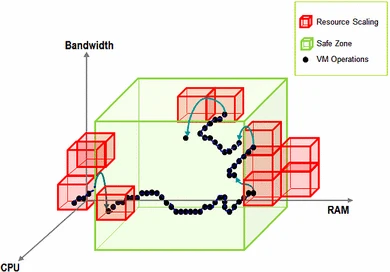
\includegraphics[scale=1.2]{img/SDTScaling.png}
  \caption{Safe-Zone and Resource Scaling Thresholds (from Paper ACCRS: autonomic based cloud computing resource scaling )}
\end{figure}

Die Grafik stellt die Safe-Zone als grünen Kasten, die Over- bzw. Under-Utilization als rote Kästchen, die an die Grenzen der Safe-Zone grenzen dar. Die X,Y und Z-Achsen, repräsentieren die Auslastung von RAM,Netzwerk und CPU. Anhand von Sprüngen, die der Graph der VM-Operations nach überschreiten der Safe-Zone Grenze zurück in die Safe-Zone macht, kann nachvollzogen werden, dass skaliert wurde und so die Last pro VM gesunken ist.

Die Skalierung in diesem Projekt orientiert sich an dem Verfahren, welches im Paper 'ACCRS: autonomic based cloud computing resource scaling' eingesetzt wird. Die Idee der Zustände Safe-Zone, Under-Utilization sowie Over-Utilization und deren Erkennung mittels statischer Regeln werden adaptiert und auf das Kubernetes-Konzept der Deployment-Skalierung übertragen, die Thresholds werden allerdings abgewandelt. 


\pagebreak
\section{Datenaggregation}

Die Datenaggregation, also das Erheben und Sammeln von Daten, ist zentraler Bestandteil des Projektes und der erste grundlegende Schritt. Das Ziel der Aggregation ist es Daten sog. Metriken über den Zustand eines Kubernetes-Clusters(siehe Kapitel Grundlagen/Kubernetes) zu erhalten. Kubernetes stellt selbst Metriken zur Verfügung, mittels eines passenden Tools werden diese ausgelesen und so für die weitere Verarbeitung nutzbar gemacht.

\subsection{Toolauswahl} <evtl. hieraus eigenes Kapitel machen,für Prometheus, Grafana,(Loki)>

Das Monitoringtool, welches in diesem Projekt zur Datenaggregation genutzt wird, ist Prometheus. Prometheus wird als Quasi-Standard im Cloud-Native Umfeld und für das Monitoring von Kubernetes verwendet <Hierfür belegende Quelle finden>. Für dieses Projekt bietet es zentrale Features, welche die Umsetzung ermöglichen.

\begin{description}

\item[Automatische Service-Discovery]
Das Feature der automatische Service-Discovery ist sehr entscheident, da sich die Services im Cluster häufig verändern und neue Services hinzugefügt werden. Mithilfe dieser Funktion werden Services automatisch gefunden, Metriken direkt erhoben und Regeln auf diese angewendet, ohne konfiguriert werden zu müssen.
\item[Echtzeitmetriken]
Prometheus zeichnet Metriken in Echtzeit auf. Das ermöglicht es jederzeit den aktuellen Status des Clusters einzusehen und in Echtzeit darauf reagieren zu können.
\item[Zeitreihen]
Prometheus zeichnet Metriken als Zeitreihen auf, was das Beobachten, Abfragen und die Definition von Regeln über Zeiträume möglich macht. 
\item[Regeln]
Regeln spielen eine zentrale Rolle in diesem Projekt. Mithilfe dieser lassen sich verschiedene Features von Prometheus regulieren, in diesem Projekt werden sie für das Regulieren von Alerts verwendet.
Regeln werden über Thresholds und optional über Zeiträume von Metriken definiert, sodass bei Überschreiten eines Thresholds für eine bestimmte Zeit eine Regel als erfült gilt.
\item[Alerting]
Mithilfe der Alerts ist es möglich anhand von Regeln Alarme zu versenden, die über den Zustand des Clusters informieren. Sie können an Ziele wie E-Mail-Adressen oder Chat-Tools wie Slack oder Telegram gesendet werden, aber auch  an selbst definierte Endpunkte um sie dort zu empfangen oder sie möglicherweise weiterzuverarbeiten.

\end{description}

\subsection{Grafana}

Grafana ist das Tool, welches zur Visualisierung verwendet wird. Das Open-Source Tool bietet Möglichkeiten Metriken in Form von Graphen, Zählern, Histogrammen und vielem mehr über Zeiträume zu visualisieren. Des Weiteren können ganze 'Dashboards' erstellt werden, die den Überblick über das ganze Cluster auf einmal erlauben.\\
Aufgrund der bereits vorhandenen Prometheusintegration ist eine Verwendung bei bereits bestehendem Prometheus-Server einfach und innerhalb kurzer Zeit umzusetzen.
Der Prometheus-Server, von welchem Grafana Metriken erhalten soll muss als Datenquelle mittels seiner Adresse konfiguriert werden, danach stehen alle Metriken, welche Prometheus kennt auch in Grafana zur Verfügung.\\
Um Metriken zu visualisieren, wird die aus Prometheus bereits bekannte Abfragesprache PromQL verwendet, was den Vorteil bietet, Abfragen die für Prometheus funktionieren, funktionieren ebenso in der Grafana Oberfläche zum erstellen von Visualisierungen.\\
Da Grafana eines der gängistens Tools ist und teilweise als Quasi-Standard zur Visualisierung von Metriken behandelt wird, findet eine kontinuierliche Weiterentwicklung statt und eine große Community bietet Unterstützung und Erfahrungen.\\<hier Quelle Logz.io einfügen>
Die Erweiterbarkeit ist ebenfalls gegeben, neben Visualisierungen für Metriken, bestehen Möglichkeiten Logs, Statistiken und vieles mehr zu Visualisieren und in Dashboards zu integrieren.

\subsection{Datenquellen}

Als Datenquelle dienen potenziell alle Ziele, die von Prometheus mittels der Target-Discovery innerhalb des Kubernetes-Cluster gefunden werden und Daten bereitstellen.\\
Von besonderem Interesse für dieses Projekt sind hierbei alle system- und hardwarenahen Targets, wie der kubelet (siehe Kapitel Grundlagen) und cAdvisor in Pods und Containern.

\subsubsection{'USE'-Methode}

Das Monitoring der Systemressourcen wird nach der 'USE'-Methode durchgeführt. Diese Methode wurde von Brendan Gregg, einem Netflix-Ingenieur im Bereich Cloud-Performance, mit Schwerpunkt auf das Monitoring von Systemressourcen entwickelt, weshalb sie sich für dieses Projekt eignet.
Ziel der Methode ist es die Utilization, der Zeitdurchschnitt der Arbeit, die eine Ressource beschäftigt erledigt, die Saturation, die "Zusatzarbeit" die eine Ressource verrichten muss, im Moment aber nicht leisten kann sowie die Error-Rate, die Häufigkeit in der Fehler auftreten von Systemkomponenten wie CPU, RAM und Netzwerkbandbreite abzubilden.

<Quelle Brendan Gregg einfügen>

\subsubsection{Metriken}

Die Metriken, mit denen die USE-Methode umgesetzt wird, werden aus den Systemmetriken, die durch Prometheus gesammelt werden, zusammengesetzt. 
Die Metriken Utilization und Saturation werden für CPU, RAM und Netzwerkauslastung folgendermaßen berechnet:

\begin{description}
\item[CPU]:\\
Utilization:\\
Die CPU Utilization berechnet sich aus der Summe der Millisekunden, welche die CPU beschäftigt war, geteilt durch eine ganze Sekunde. So erhält man die Utilization pro Sekunde, welche über aufsummiert und der Mittelwert über den beobachteten Zeitraum gebildet wird, um so die durchschnittliche Utilization zu erhalten.\\
Saturation:\\
Die CPU Saturation kann anhand des Ressourcenlimits berechnet werden. In UNIX basierten Betriebssystemen gibt es die Metrik 'load-average', welche die Anzahl der laufenden sowie wartenden Prozesse enthält. Sofern man diese durch die Anzahl der zur Verfügung stehenden CPU-Kerne teilt, erhält man eine Kennzahl für die Saturation. Diese aufsummiert und über die Zeit gemittelt, ergibt die durchschnittliche Saturation.\\
Ein weiterer Weg die Saturation zu berechnen ist das aufsummieren der Zeit in der ein Prozess 'throtteld' läuft. Dies funktioniert dann, wenn ein Prozess ein Ressourcenlimit besitzt, übersteigt er dieses wird der Prozess gedrosselt.\\
\item[RAM]:\\
Utilization:\\
Die RAM Utilization berechnet sich aus der Menge des vom System reservierten Speichers, der durch die Menge des gesamten Speichers geteilt wird. Beide stehen in UNIX basierten Betriebssystemen zur Verfügung, sodass die Rechnung zur RAM-Utilization $1 - reservierterSpeicher / gesamterSpeicher$ ist.\\
Saturation:\\
Die RAM Saturation kann am besten berechnet werden, wenn Ressourcenlimits existieren. Unter diesen Voraussetzungen kann die Saturation berechnet werden, indem die Summe des aktuell verwendeten Speichers durch das Ressourcenlimits geteilt wird.\\
\item[Netzwerk-Bandbreite]:\\
Utilization:\\
Um die Netzwerk Utilization zu messen werden die Bytes aufsummiert, die versendet sowie empfangen werden.\\
Saturation:\\
Die Netzwerk Saturation kann nur dann sinnvoll gemessen werden, wenn das Bandbreitenlimit bekannt ist. Sofern dies der Fall ist kann die Saturation berechnet werden indem die versendeten bzw. empfangenen Bytes durch das Bandbreitenlimit geteilt wird. \\
Sofern keine Information zum Limit zur Verfügung stehen, können die verworfenen Pakete (dropped Packages) als Indikator dafür dienen, wie hoch die Saturation ist.
\end{description}

\section{Auswerten der Metriken}

Das Auswerten der Metriken erfolgt für das Monitoring durch das Umsetzen der USE-Methode, beschrieben in Kapitel vier, statt.

\subsection{Klassifizierung}

Die Metriken werden in Node-Level sowie Pod- und Containerlevel Metriken klassifiziert.\\
Nodelevelmetriken repräsentieren den Zustand eines ganzen Nodes, das bedeutet, dass die Metriken die Summe aller Pods, Container, Services, etc. des Nodes darstellen.\\
Podlevelmetriken hingegen repräsentieren den Status eines einzelnen Pods sowie des Containers bzw. den Containern die sich in diesem Pod befinden.\\

\subsection{Logische Auswertung}

Die logische Auswertung der Metriken findet an zwei Stellen in diesem Projekt Anwendung. Einmal zum Erstellen von Alerting-Regeln auf dem Prometheus-Server und einmal zur grafischen Darstellung der Metriken in der Grafana-Oberfläche. In beiden Fällen wird zur Auswertung die PromQL-Sprache verwendet.
Zur logischen Auswertung werden die von Prometheus aggregierten Daten verwendet. Für das Monitoring werden die Schritte der USE-Methode Utilization, Saturation und Error-Rate jeweils für CPU, RAM sowie Netzwerk umgesetzt(siehe Kapitel vier,Metriken). Diese Metriken werden jeweils über einen Zeitraum von fünf Minuten beobachtet und ausgewertet und deren Mittelwert gebildet. Dies hat zur Folge, dass Ausreißer in der Last nicht schwer ins Gewicht fallen und so starke Schwankungen verhindert werden, was zur Verbesserung der Beobachtbarkeit beiträgt.\\
Die Auswertung der Daten zum automatische Alerting greift nicht direkt auf eine Methode wie USE zurück, orientiert sich aber an ihr. Hierfür werden die Metriken der Methode zu CPU, RAM und Netzwerk kombiniert und an Grenzwerte geknüpft um so gewünschte Grenzen abzufragen und die Regeln erfüllbar bzw. nicht erfüllbar machen zu können. Ebenso wie beim Monitoring werden auch hier die Metriken über einen Zeitraum von fünf Minuten beobachtet.\\

Nachdem die Metriken ausgewertet sind können sie nun graphisch aufbereitet werden. <Frage, sind solche Übergänge gut/hilfreich ?>

\subsection{Graphische Aufbereitung}

Zur Visualisierung der Metriken stehen in der Grafana-Oberfläche verschiedene Möglichkeiten zur Verfügung. Da es das Ziel ist möglichst auf einen Blick, den Systemressourcenzustand des ganzen Clusters sehen zu können, wird ein Dashboard mit allen USE-Metriken erstellt. Die Metriken können als Graph, Zähler, Balkendiagramm oder Heat-Map dargestellt werden.\\
Da schnell erkennbar sein soll, an welcher Stelle ungewöhnliche oder kritische Werte auftreten, werden die Zähler als Visualisierungsmethode für alle Metriken gewählt. Hierbei steht pro Metrik ein eigener Zähler zur Verfügung, womit sich der Zustand jeder Ressource einzeln einsehen lässt.\\
Für die Counter werden grüne Bereiche für unkritische Auslastung und rote Bereiche für kritische Auslastung mit einen Grenzwert von 75\% eingerichtet, um kritische Zustände hervorzuheben.
\pagebreak
\section{Automatisierte Aktionen}
\subsection{Wahl der Sprache}
\subsection{Aktionen}
\subsubsection{Skalieren}
\subsubsection{Anomalie-Detection}
\subsection{Komponenten und Architektur}
\subsubsection{Prometheus}
\subsubsection{Alertmanager}
\subsubsection{Alert-Action-Manager}
\subsection{Regeln}
\subsubsection{Metriken}
\subsubsection{Grenzwerte}

\section{Evaluation}
\subsection{Messaufbau}
\subsection{Regeln}
\subsection{Grenzwerte}
\subsection{Komponenten und Architektur}

\section{Diskussion}
\section{Fazit und Ausblick}

\newpage
\bibliography{Literatur}

\end{document}